%!TEX root = main.tex

\section{Introduction}
In recent years much effort has been put to equip GEO satellites with electric propulsion (EP) in order to reduce the mass at launch \cite{goebel2002performance} and consequently to achieve economical benefits. 
%The first task of EP was to accomplish 
Initially, EP was to accomplish
secondary maneuvers, i.e., orbital control, then its implementation culminated with satellite 702SP by Boeing, the first all-electric GEO platform (2015)\footnote{Data from \url{http://www.absatellite.net/wp-content/uploads/2015/09/ABS-3A-Enters-Service-10-Sep-2015-FINAL.pdf}}. 
% * <francesco.topputo@gmail.com> 2016-09-04T06:41:18.870Z:
%
% (Mi riferivo a i.e. ed e.g.)
%
% ^ <francesco.topputo@gmail.com> 2016-09-06T19:12:41.363Z.
% * <francesco.topputo@gmail.com> 2016-09-04T06:40:10.776Z:
%
% Vale la stessa cosa di GEO. Non c'è bisogno di usare il corsivo (che in generale non deve essere abusato).
%
% ^ <francesco.topputo@gmail.com> 2016-09-06T19:12:43.251Z.
Low-thrust propulsion has produced a shift of the initial orbit, from the classical Geostationary Transfer Orbit (GTO) to the more customized Supersynchronous Transfer Orbit (SSTO) \cite{pooleboeing}, in pursuance to decreasing the high time-of-flight (often many months), typical of the EP.
The more classical strategy to place a satellite in GEO relies on chemical propulsion (CP)\cite{wertz2011space}. Even if this path is more expensive than the latest one, it guarantees a very short transfer time, often few days starting from the GTO.
This dichotomy is shown in \figurename\ref{fig:dichotomy}, where the Fully-Chemical Transfer (FCT) and the Fully-Electric Transfer (FET) are outlined.
\begin{figure}[htp]
\centering
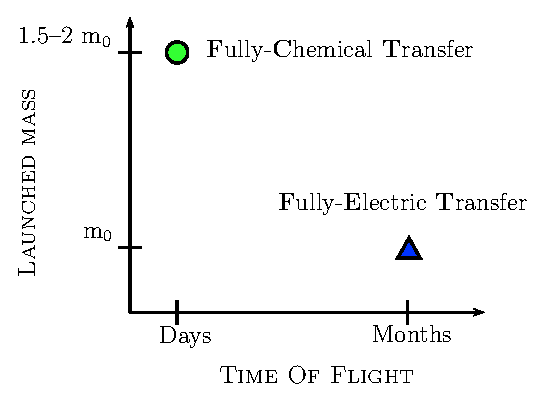
\includegraphics[width=0.5\textwidth]{cartesian_FCFE.eps}
\caption{\textbf{GEO transfer dichotomy}}
\label{fig:dichotomy}
\end{figure}
\\
Communication satellites have the lion's share in the GEO market\footnote{Data retrieved from UCS Satellite Database.}, which represents a very profitable business\footnote{Data retrieved from "State of the satellite industry report-June 2016", Satellite Industry Association (SIA) \url{http://www.sia.org/wp-content/uploads/2016/06/SSIR16-Pdf-Copy-for-Website-Compressed.pdf}}.
% * <francesco.topputo@gmail.com> 2016-09-04T06:50:27.728Z:
%
% > This dichotomy is shown in \figurename\ref{fig:dichotomy}, where the Fully-Chemical Transfer (FCT) and the Fully-Electric Transfer (FET) are outlined.
% > \begin{figure}[htp]
% > \centering
% > 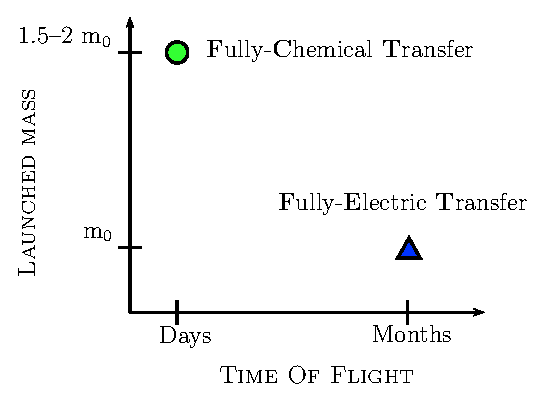
\includegraphics[width=0.4\textwidth]{cartesian_FCFE.eps}
% > \caption{\textbf{GEO transfer dichotomy}}
% > \label{fig:dichotomy}
% > \end{figure}
% > \\
%
% Nella tesi avevamo una figura leggermente diversa di questa (ricordo di avere suggerito una modifica sull'asse y)
%
% ^ <francesco.topputo@gmail.com> 2016-09-06T19:13:20.838Z:
%
% Ok, ma perche' le scritte FCT e FET si sono ingigantite? 
%
% ^.
It is easy to notice the lack of a mission plan that assures a lower propellant consumption than the FCT while still having transfer times shorter than those of FET.

Studies by various authors proposed combining both CP and EP to have these intermediate features.
\citeauthor{oleson1996launch}~\cite{oleson1996launch}, using SEPSPOT~\cite{sackett1975solar} demonstrated the reduction of launch vehicle net mass with high launch latitudes and Solar Electric Propulsion (SEP).~\citeauthor{Mailhe:2002aa}~\cite{Mailhe:2002aa} considered a vehicle design for a coplanar transfer from LEO to GEO equipped with both chemical and electric propulsion. The aim was to reduce the total radiation loads on the spacecraft and to provide attractive total trip times.~\citeauthor{corey2010performance}~\cite{corey2010performance} provided a system analysis of a large communication satellite equipped with SEP; they summarized the Space System Loral experience with an Hall-Effect-Thruster (HET) qualification and discussed the benefits of Electric Orbit Raising (EOR) to reach Geostationary Equatorial Orbit.~\citeauthor{Kluever:2012aa}~\cite{Kluever:2012aa} contributed to all these works with a comprehensive analysis of GEO insertion with the Combined Chemical- Electric Propulsion (CCEP) concept. The approach relied on only six free design variables, and realistic effects, such as eclipses and power degradation, were considered.  Furthermore,~\citeauthor{Kluever:2015aa}~\cite{Kluever:2015aa} provided an algorithm to rapidly perform trade studies for transfers using chemical and electric propulsion. The starting variables were the mass delivered in GEO, the desired transfer time, and a desired electric propulsion system. Eclipses were not considered during the transfer.

Previous works show the main difficulties while dealing with this research field, such as the low-thrust trajectory optimization, the inclusion of realistic effects on both the Earth and the space environment, and, last but not the least, providing achievable and acceptable results while using reasonable amount of computational time and memory. In attempting to prove the advantage of these \textit{hybrid} systems, recent studies revealed that hybrid platforms have peculiar features when applied to missions to the Moon \cite{kluever1997optimal,mingotti2012hybrid}, Mars, and NEOs, by \cite{esa-prof}.

This paper elaborates on the concept of Hybrid Transfer (HT), which involves using both CP and EP operating at different times. In our view, FCT and FET are special solution of the HT family. This new family of design solutions is produced by a different balancing of CP and EP. The goal is widening the trade space for GEO missions by providing a set of solutions with varying transfer time and launched mass.
% * <francesco.topputo@gmail.com> 2016-09-04T07:21:20.487Z:
%
% > This paper elaborates on the concept of Hybrid Transfer (HT), which involves using both CP and EP operating at different times. In our view, FCT and FET are special solution of the HT family. This new family of design solutions is produced by a different balancing of CP and EP. The goal is widening the trade space for GEO missions by providing a set of solutions with varying transfer time and launched mass.
%
% Ho commentato la figura con la barra orizzontale. Possiamo ometterla (non ho controllato che non fosse più citata nel testo)
%
% ^ <francesco.topputo@gmail.com> 2016-09-06T19:13:30.378Z.
% \begin{figure}[htp]
% \centering
% 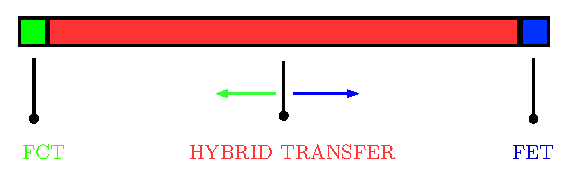
\includegraphics[width=0.4\textwidth]{family.eps}
% \caption{\textbf{Abstraction of Space transfer solutions}}
% \label{fig:abstractionofspacetransfersolutions}
% \end{figure}
% \\
At the same time, a new and fast method for mission and systems design is developed, together with a cost analysis to assess the economic benefits of the HT.
These involve high-thrust and low-thrust trajectories analyses, power subsystem sizing, electric and chemical propulsion modeling based on real performances of the thrusters.
The preliminary mission and system design is combined with the solar-cell degradation analysis due to passage through radiation belts (Van Allen Belts). 
The work required a multidisciplinary approach where, although the in the preliminary stages, the academic part and the applied satellite operation are equally important.

The paper is organized as follows. In Sec.\ref{sec:missionalaysis} the low-thrust/high-thrust trajectories and the spacecraft configuration are analyzed, thus showing how the combination of CP and EP are managed. In Sec.\ref{sec:spacecraftsystemdesign} the technology of chemical and electric propulsion are detailed, dealing with the spacecraft systems design and the modeled subsystems. Sec.\ref{sec:costanalysis} explains how a preliminary, approximated economic analysis is performed to assess the advantages of a Hybrid Transfer from an overall cost point of view. In Sec.\ref{sec:solutionpath}, the solution method is explained, and the fundamental steps are described, while in Sec.\ref{sec:results} a case study is presented together with a critical discussion of the results obtained.